\documentclass[runningheads,a4paper]{llncs}

\usepackage[utf8]{inputenc}
\usepackage[T1]{fontenc}
%\usepackage[ngerman]{babel}
\usepackage{enumerate}
\usepackage{listings}
\usepackage{marvosym}
\usepackage{gensymb}
\usepackage[bookmarks,bookmarksopen,bookmarksdepth=2]{hyperref}
\usepackage{amsmath}
\usepackage{amsfonts}
\usepackage{amssymb}
%\usepackage{amsthm}
\usepackage{mathrsfs}
\usepackage{fancyhdr}

\usepackage{graphicx}
\graphicspath{{./img/}}

\usepackage[acronym,toc]{glossaries}
\makeglossaries

%%%%%%%%%%%%%%%%%%%%%%%%%%%%%%%%%%%%%%%%%%%%%%%%%%%%%%%%%%%%%%%%%%%%%%%%%

%\newtheorem{definition}{Definition}
%\newtheorem{theorem}{Theorem}
\newtheorem{axiom}{Axiom}


\newcommand{\partOf}{~\textsf{partOf}~}
\newcommand{\properPartOf}{~\textsf{properPartOf}~}
\newcommand{\atomOf}{~\textsf{atomOf}~}
\newcommand{\fragmentOf}{~\textsf{fragmentOf}~}
\newcommand{\atomicFragmentOf}{~\textsf{atomicFragmentOf}~}
\newcommand{\correspondsTo}{~\textsf{correspondsTo}~}
\newcommand{\correspondsToR}[1]{~\textsf{correspondsTo}_{#1}~}
\newcommand{\conformsTo}{~\textsf{conformsTo}~}

\newcommand{\footnoteurl}[1]{\footnote{\url{#1}}}

\newcommand{\megal}{\text{MegaL}}
\newcommand{\megalxtext}{\text{MegaL/Xtext}}
\newcommand{\megaltext}{\text{MegaL/Text}}
\newcommand{\eclipse}{\text{eclipse}}
\newcommand{\thesis}{Megamodel-driven Traceability Recovery \& Exploration in an O/R/X-Mapping scenario along the mereological aspects of software artifacts}


%%%%%%%%%%%%%%%%%%%%%%%%%%%%%%%%%%%%%%%%%%%%%%%%%%%%%%%%%%%%%%%%%%%%%%%%%

\title{Exposé for B.Sc. Thesis}
\subtitle{\thesis}
\author{Maximilian Meffert\\210101205}
\institute{University of Koblenz-Landau}

\begin{document}


\maketitle
%
%\begin{abstract}
%asdf 
%\end{abstract}


\section{Introduction}
This exposé\footnote{\url{http://www.softlang.org/info:expose}} outlines the thesis:
\begin{center}
\it
\thesis
\end{center}
for acquiring the degree Bachelor Science (B.Sc.) in Computer Science.

The central topic of the thesis will be the study of \megal's traceability capabilities.


\subsection{Road-map}
Section \ref{section:Motivation} motivates the topic of the thesis.
\ref{section:Background} gives a short overview over the necessary background information.
\ref{section:ResearchHypthesesAndQuestions} defines a preliminary hypothesis and formulates the research questions.
\ref{section:Objectives} specifies the important objectives for the thesis.
\ref{section:Methodology} describes the approach and methodology of the thesis.
Eventually \ref{section:StructureOfTheThesis} outlines the interim structure of the thesis.


\section{Motivation}
\label{section:Motivation}
A common task during the development of software systems is to persist and serialize a domain model.
For instance, consider a simple web-service where data is stored in a database and served via HTTP in serialized form, e.g. XML.

\begin{figure}[h!]
\centering
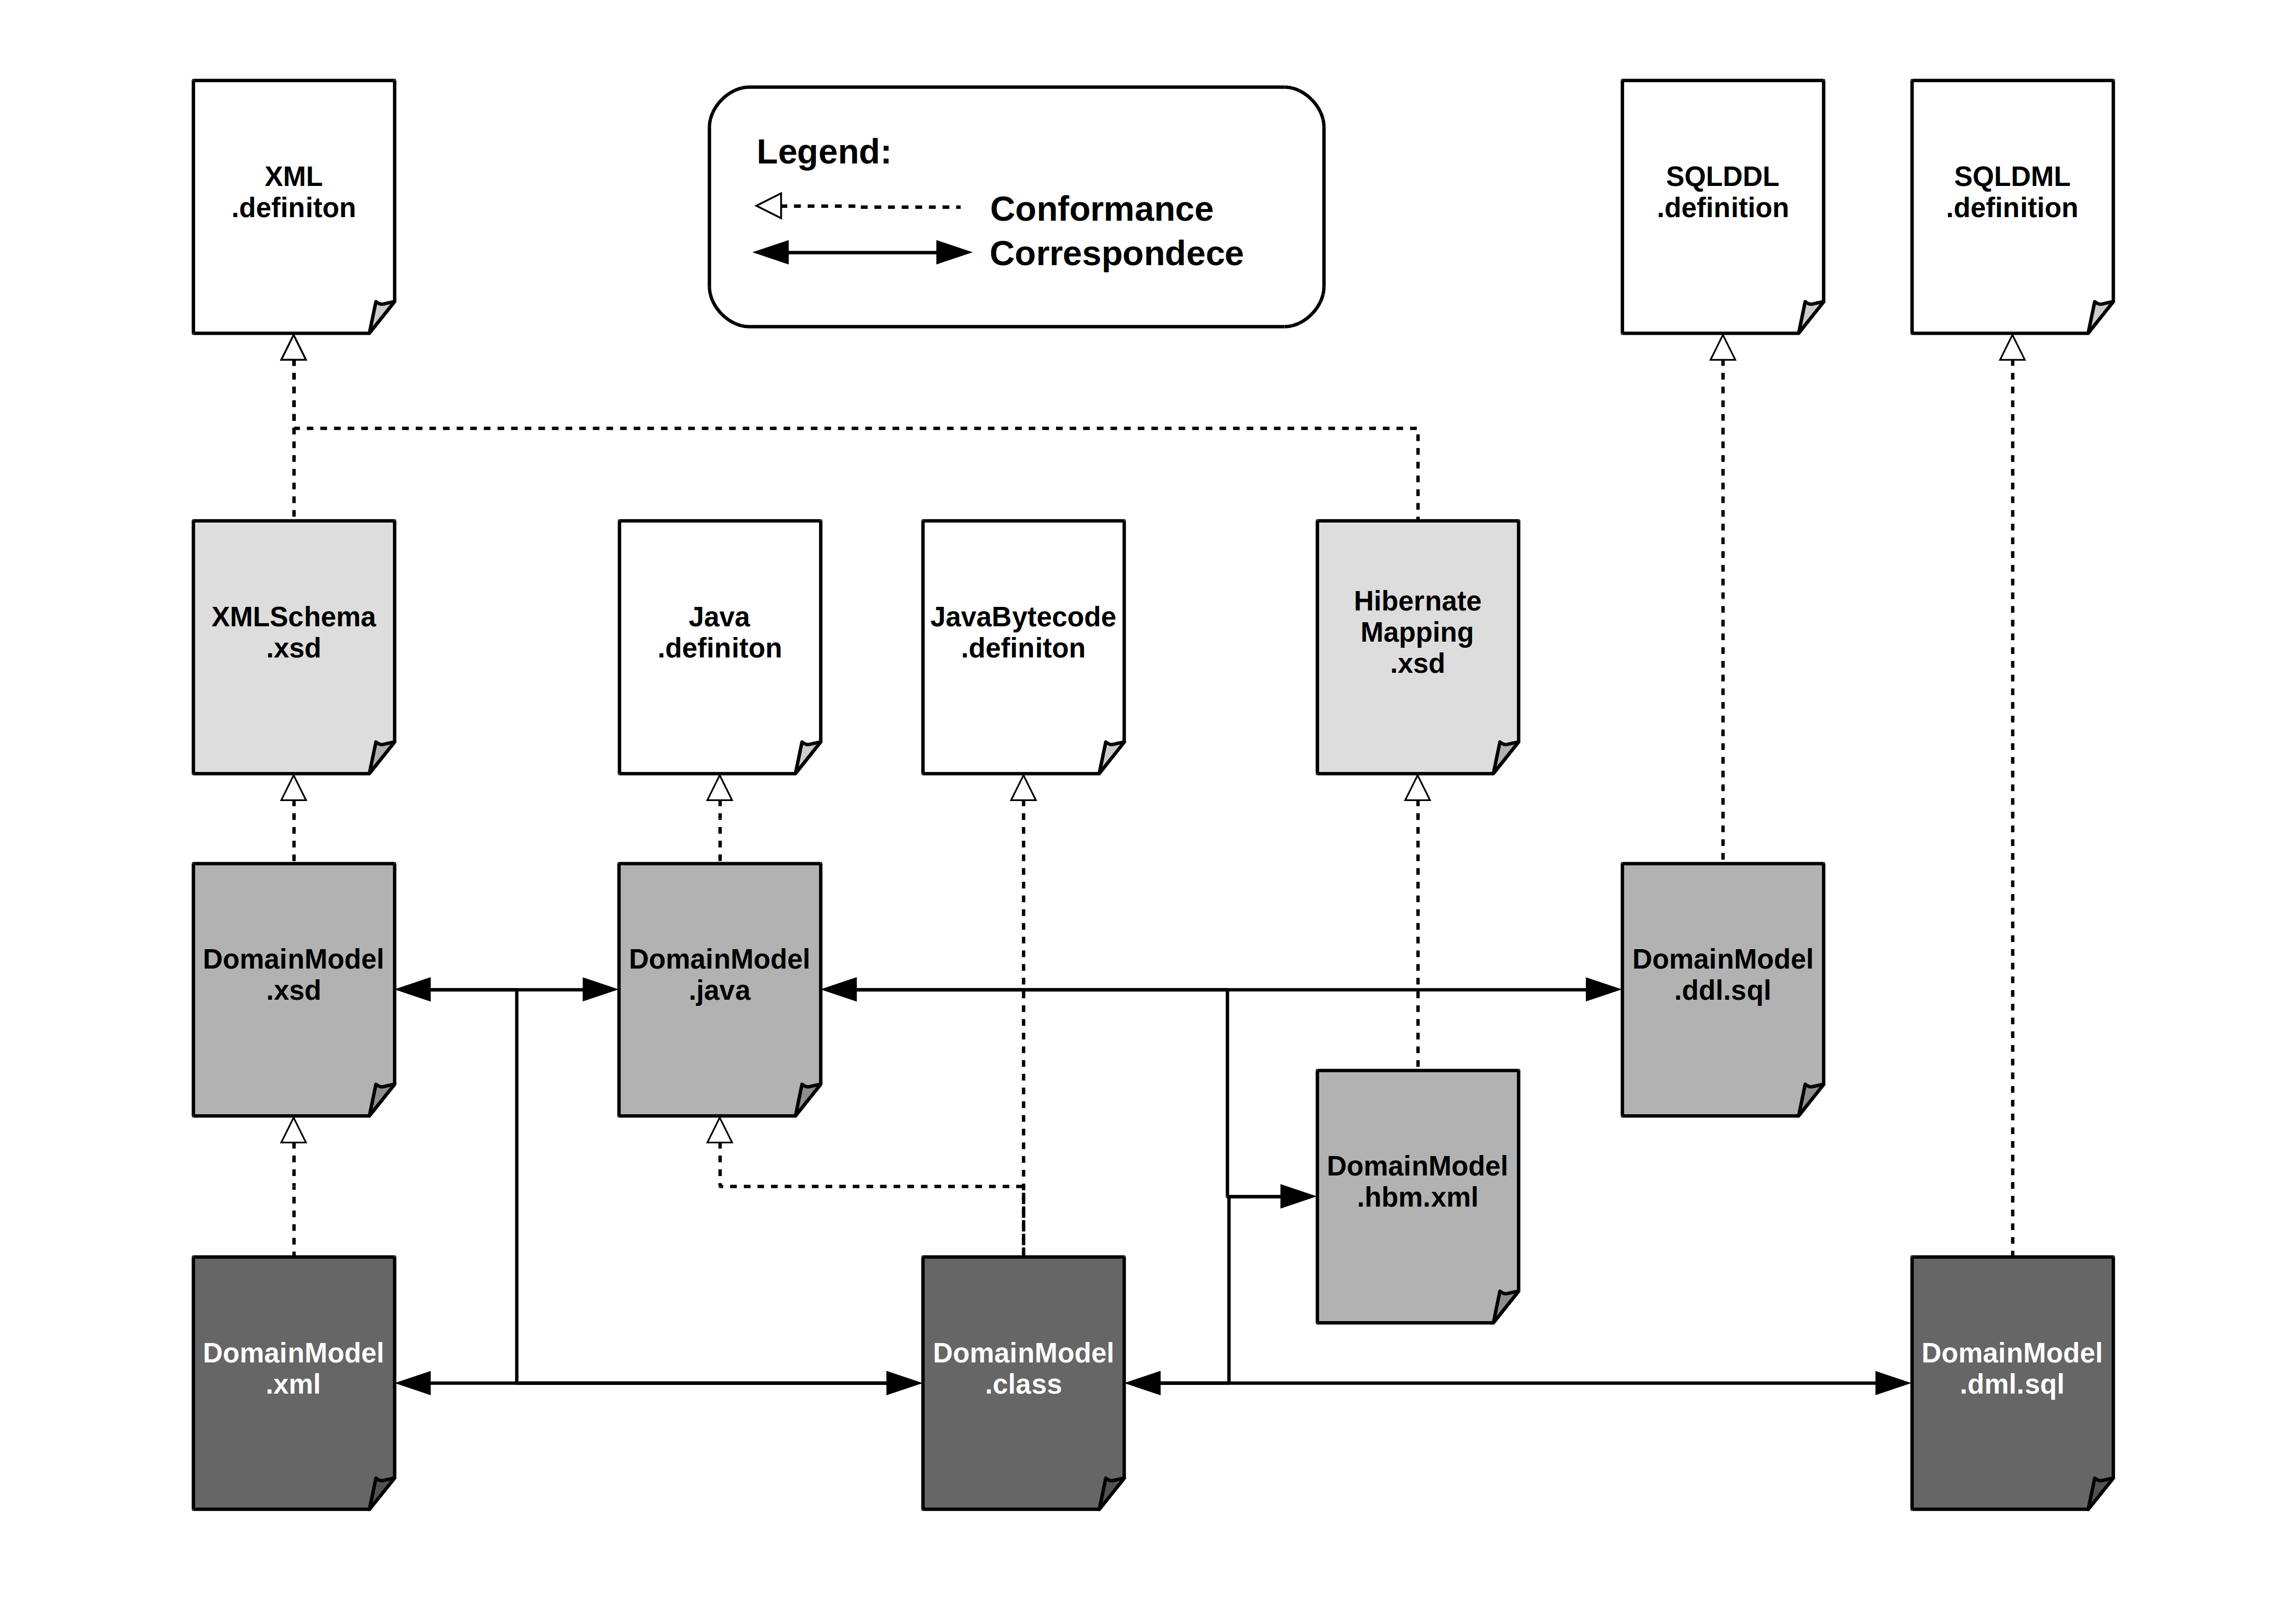
\includegraphics[width=.9\textwidth]{orx-correspondence-big-picture.png}
\caption{O/R/X-Correspondence}
\label{figure:ORXCorrespondenceBigPicture}
\end{figure}

\begin{table}[h!]
\resizebox{\textwidth}{!}{
\begin{tabular}{l|l|l}
&& \\
\textbf{Language} 
&\textbf{Fragment Type}
&\textbf{Fragment Text}
\\ && \\ \hline && \\
Java
&Class Property
&\texttt{public String name;}
\\ && \\
XSD 
&Attribute Definition
&\texttt{<xs:attribute name="name" type="xs:string"/>}
\\ && \\
XML
&Attribute
&\texttt{name="Alan Turing"}
\\ && \\
Hibernate XML
&Property Mapping
&\begin{minipage}{\columnwidth}
\ttfamily
<property access="field" generated="never" lazy="false" name="name" optimistic-lock="true" type="java.lang.String" unique="false">
\\\hspace*{0.1\columnwidth}<column name="name"/>
\\</property>
\end{minipage}
\\ && \\
SQL/DDL
&Column Definition
&\texttt{`name` varchar(255) DEFAULT NULL,}
\\ && \\
\end{tabular}
}
\newline
\caption{O/R/X-Correspondence}
\label{table:ORXCorrespondenceExample}
\end{table}




\section{Background}
\label{section:Background}
The thesis will be based but is not limited to aspects of the following topics:

\subsection{Ontologies}
\subsection{Traceability}

\subsection{Mereology}
Mereology is the systematic study of the relationships between wholes and part \cite{DBLP:journals/dke/Varzi96}.
The core of its discourse is the Parthood- or \partOf-Relationship, which is axiomatized as follows:
\begin{definition}[\partOf]
We denote:
\begin{align*}
x \partOf y
\end{align*}
and mean that $x$ is constituent for $y$.
We assume that:
\begin{itemize}
\item[P1] $x \partOf x$ (Reflexiveness)
\item[P2] $x \partOf y \wedge y \partOf x \Rightarrow x = y$ (Antisymmetry)
\item[P3] $x \partOf y \wedge y \partOf z \Rightarrow x \partOf z$ (Transitivity)
\end{itemize}
\end{definition}




\subsection{Megamodelinng (with \megal)}
\megal\footnoteurl{http://www.softlang.org/megal/} is a Domain Specific Language (DSL) and technology designed  for modeling the linguistic architecture of software systems.
It is actively developed by the Software Language Team\footnote{\url{http://www.softlang.org/}} at the University of Koblenz-Landau and currently has two implementations: 
\begin{itemize}
\item
\megalxtext an \eclipse based Integrated Development Environment (IDE)
\item
and \megaltext a text-file and console based implementation with an 
\end{itemize}

\subsection{Program Analysis}
Program Analysis is the process of automatically analyzing programs.
This can be done (a) statically by analyzing the source code of a program or (b) dynamically through monitoring and intercepting the runtime of a program, analyzing transient artifacts. 


\subsection{XML Data Binding (with JAXB)}
XML Data Binding is the process of automatically mapping instance- and model-level objects into a XML-serialized form.
That is, for the Java Architecture for XML Binding (JAXB)\footnoteurl{https://docs.oracle.com/javase/tutorial/jaxb/intro/arch.html}, a Java class itself is mapped via annotations to an XML Schema, both model-level objects.
With this mapping Java class-instances can easily be de-/serialized into XML Documents, a process called un-/marshaling.
XML Data Binding allows to directly work with a domain model rather than working with direct XML access.

\subsection{Object-Relational Mapping (with JPA/Hibernate)}
Object-Relational Mapping is the process of automatically mapping instance- and model-level objects into a relational data-storage.
In case of SQL-database technologies, model-level objects are mapped to SQL/DDL (Data Definition Language) statements and instance-level objects are mapped to SQL/DML (Data Manipulation Language) statements.
Usually, these statements are then sent to and executed by a SQL-database server.
This allows to directly work with a domain model when persisting data.

The Java Persistence API (JPA)\footnoteurl{http://www.oracle.com/technetwork/articles/javaee/jpa-137156.html} is a Java standard interface for working with Object-Relational Mapping.
Hibernate\footnoteurl{http://hibernate.org/} is one of many JPA implementations.
It provides annotations and a XML Schema for defining Object-Relational Mappings between Java classes and database tables.

\section{Research Hypotheses \& Questions}
\label{section:ResearchHypthesesAndQuestions}
\subsection{Research Hypotheses}
\subsubsection{Correspondence}
\cite{DBLP:conf/sle/Lammel16} axiomatizes a strict one-to-one correspondence of software artifacts as follows:
Given there is an arbitrary relationship $R$ between to languages $L_1$ and $L_2$:
\begin{align*}
R : L_1 \times L_2
\end{align*}
For instance, $R$ may be a transformation from one language to the other.

Then two artifacts $a_1 \in L_1$ and $a_2 \in L_2$ correspond to each other only if for each part of one artifact there exists exactly one corresponding part of the other:
\begin{align*}
&(a_1,a_2) \in R
\\&\wedge \forall b_1 \in L_1 : b_1 \partOf a_1 \Rightarrow (\exists! b_2 \in L_2 : b_2 \partOf a_2 \wedge b_1 \correspondsToR{R} b_2 )
\\&\wedge \forall b_2 \in L_2 : b_2 \partOf a_2 \Rightarrow (\exists! b_1 \in L_1 : b_1 \partOf a_2 \wedge b_2 \correspondsToR{R} b_1 )
\\&\Rightarrow a_1 \correspondsToR{R} a_2
\end{align*}

However, \cite{DBLP:conf/sle/Lammel16} also notes that this kind of correspondence may be unrealistic since real world artifacts may contain two or more parts corresponding to only one part in another artifact, e.g. an XSD documents can contain an element and a complex type definition corresponding to only on Java class declaration.
For this reason the thesis will assume a weaker correspondence hypothesis.

\subsubsection{Fragment Correspondence Hypothesis}
One objective of the thesis should be to provide empirical assurance for the axiom above in the sense that correspondence is in fact mereologically induced.
So if two artifacts $a_1$ and $a_2$ are assumed to correspond to each other, e.g. $a_2$ could be the result of a transformation of $a_1$, then parts of both artifacts should exist which also correspond to each other.
\begin{align*}
&\forall a_1 \in L_1, a_2 \in L_2 : 
a_1 \correspondsToR{R} a_2
\\&\Rightarrow 
\exists b_1 \in L_1, b_2 \in L_2 : 
b_1 \partOf a_2 \wedge b_2 \partOf a_2 \wedge b_1 \correspondsToR{R} b_2
\end{align*}

%Because the thesis will conduct empirical examination with real world artifacts, the hypothesis can be refined.
%two helpful predicates can be defined:
%\begin{align*}
%x \properPartOf y &:\Leftrightarrow x \partOf y \wedge \neg (y \partOf x)
%\\x \atomOf y &:\Leftrightarrow x \properPartOf y \wedge \neg \exists z(z \properPartOf x)
%\\x \fragmentOf y &:\Leftrightarrow x,y \in L \wedge x \properPartOf y
%\\x \atomicFragmentOf y &:\Leftrightarrow x,y \in L \wedge x \atomOf y
%\end{align*}
%\begin{align*}
%&a_1 \correspondsToR{R} a_2
%\wedge f_1 \atomicFragmentOf a_1
%\wedde f_2 \atomicFragmentOf a_2
%\\&\Rightarrow 
%(f_1, f_2) \in R
%\end{align*}
%where \properPartOf is a standard irreflexive parthood relationship from \cite{DBLP:journals/dke/Varzi96}, and \fragmentOf
%If two artifacts are in a Correspondence-Relationship, they contain constituent parts in the same relation to each other, i.e.:
%\begin{align*}
%&\forall a_1 \in L_1, a_2 \in L_2 (a_1 \correspondsToR{R} a_2
%\\&\Rightarrow
%\exists f_1, f_2: 
%f_1 \fragmentOf a_1 
%\wedge f_2 \fragmentOf a_2 
%\wedge f_1 \correspondsToR{R} f_2)
%\end{align*}
\subsubsection{Fragment Conformance Hypothesis}
If two artifacts are in a Conformance-Relationship, they contain constituent parts in the same relation to each other, i.e.:
\begin{align*}
&A_1 \conformsTo A_2
\\&\Rightarrow
\exists a_1, a_2: 
a_1 \partOf A_1 
\wedge a_2 \partOf A_2 
\wedge a_1 \conformsTo a_2
\end{align*}

\subsection{Research Questions}
Research Questions are:
\begin{itemize}
\item[RQ1] description
%\item[RQ2] description
%\item[RQ3] description
\end{itemize}

\section{Objectives}
\label{section:Objectives}
Objectives for the thesis are:
\begin{itemize}
\item[O1]
Implementation of a \megalxtext-extension capable of recovering traceability links representing PartOf-, Correspondence- and Conformance-Relationships between code fragments.
\item[O2]
Implementation of a \megalxtext-extension allowing for an user to visually explore traceability links, i.e. PartOf-, Correspondence- and Conformance-Relationships between code fragments.
\item[O3]
Providing an extensive discussion comparing \megal with related approaches on traceability recovery.
\item[O4]
Providing an extensive discussion comparing \megal with related approaches on ontologies for software artifacts or software engineering in general.
%\item[O5] description
%\item[O6] description
\end{itemize}

\section{Methodology}
\label{section:Methodology}
Thesis and research will utilize an example-driven approach inspired by the 101system\footnoteurl{https://101wiki.softlang.org/101system}.
For this, the system to study will be an imaginary Human Resource Management System (HRMS).
Figure \ref{figure:TheCompanyModel} shows an UML-Class-Diagram depicting the model of this system.

\begin{figure}[h!]
\centering
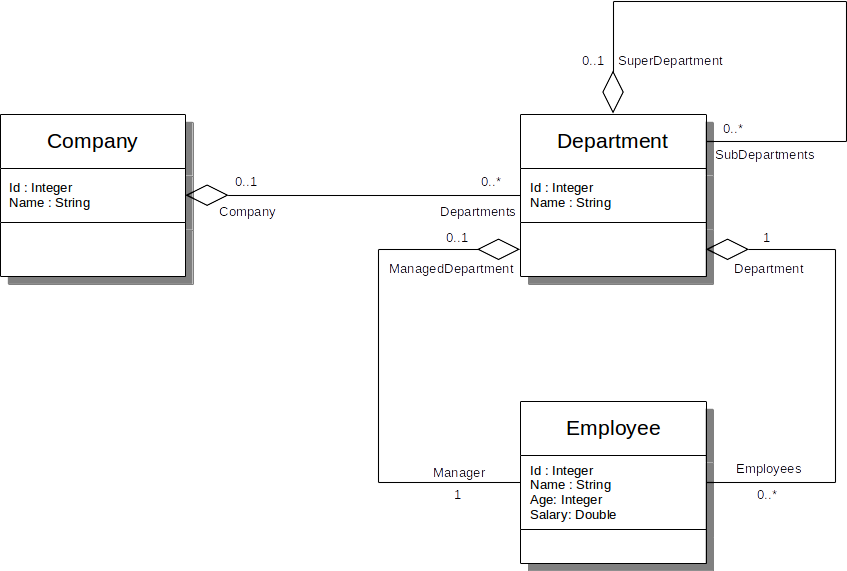
\includegraphics[width=.6\textwidth]{companies.png}
\caption{The Human Resource Management System Model}
\label{figure:TheCompanyModel}
\end{figure}

\noindent
This HRMS will be implemented in plain Java with two scenarios in mind:
\begin{enumerate}
\item 
XML-Binding with JAXB
\item
Persitence with JPA/Hibernate
\end{enumerate}
Both scenarios will be studied with the concrete instance of the HRMS model depicted in figure \ref{figure:TheCompanyInstanceCalledSoftlangInc}.

\begin{figure}[h!]
\centering
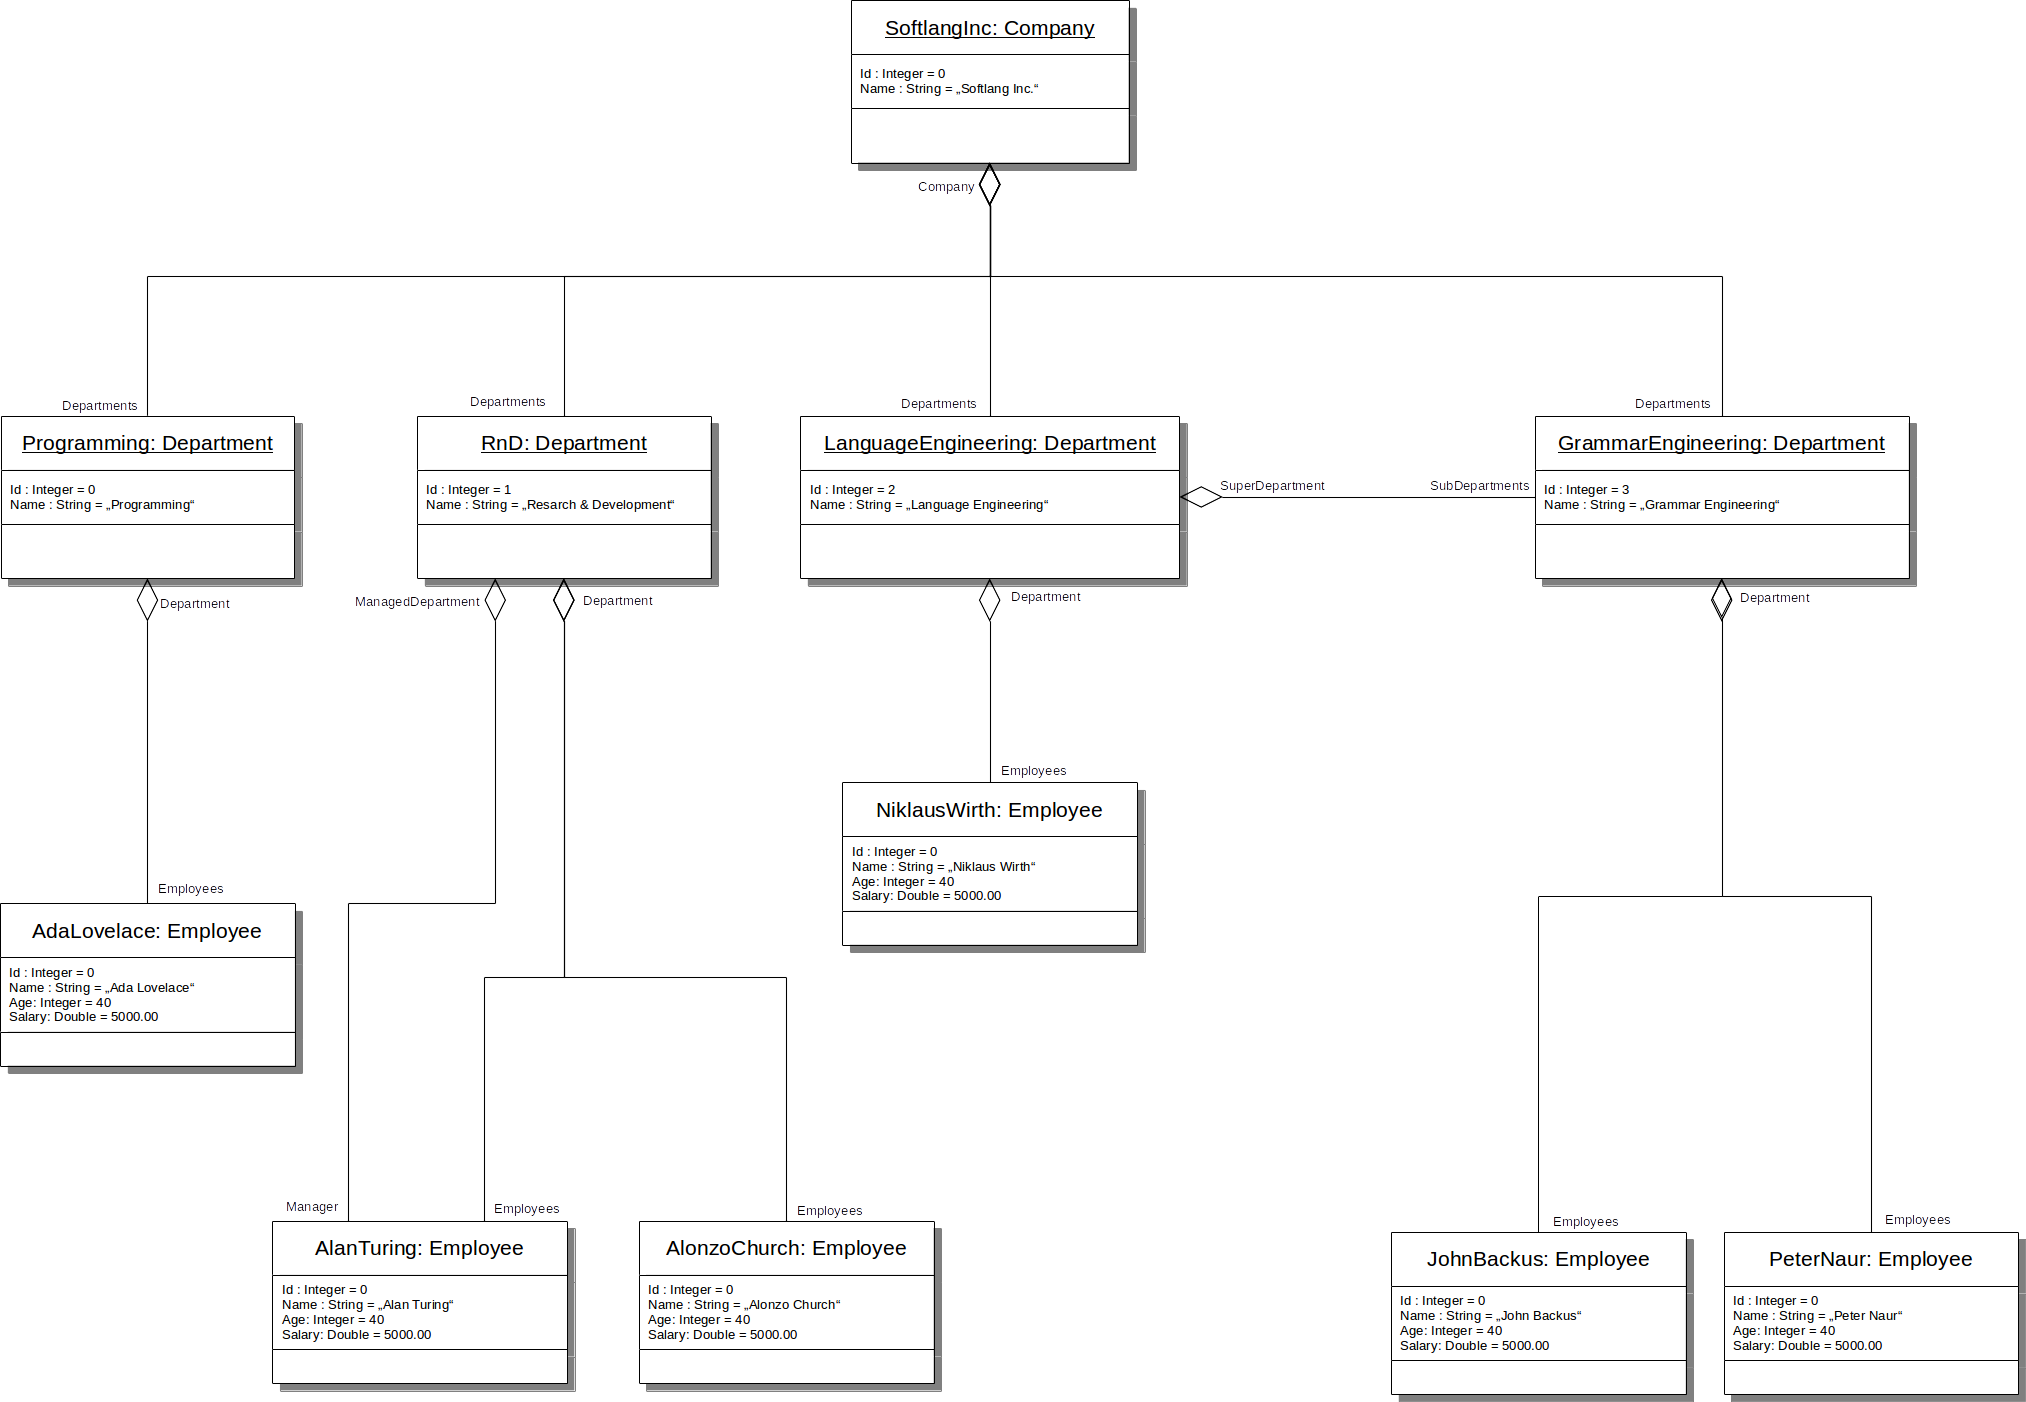
\includegraphics[width=.9\textwidth]{softlanginc.png}
\caption{The Human Resource Management System Instance called \textit{Softlang Inc.}}
\label{figure:TheCompanyInstanceCalledSoftlangInc}
\end{figure}

\section{Structure of the Thesis}
\label{section:StructureOfTheThesis}
The interim structure\footnoteurl{http://softlang.wikidot.com/info:thesis-structure} of the thesis is depicted in figure \ref{figure:StructureOfTheThesis}.
\ref{figure:TheCompanyModel}

\begin{figure}[h!]
\begin{center}
\begin{minipage}[t]{0.5\textwidth}
\begin{enumerate}

\item
\textbf{Introduction}

\item
\textbf{Background}

\item
\textbf{Related Work}

\item
\textbf{Methodology}

\item
\textbf{Requirements}

\item
\textbf{Design}

\item
\textbf{Implementation}

\item
\textbf{Case Study}

\item
\textbf{Analysis/Results}

\item
\textbf{Conclusion}

\end{enumerate}
\end{minipage}
\end{center}
\caption{Structure of the Thesis}
\label{figure:StructureOfTheThesis}
\end{figure}





\cite{DBLP:conf/ecmdafa/LammelV14}
\cite{DBLP:conf/models/FavreLV12}
\cite{DBLP:journals/dke/Varzi96}
\cite{DBLP:journals/entcs/FavreN05}
\cite{Softlang:course/ptt15/technoloymodeling}
\cite{DBLP:conf/sle/Lammel16}

\bibliographystyle{splncs}
\bibliography{../bsc}{}

%\printglossaries
%\printglossary[type=\acronymtype]

\end{document}
